\documentclass{article}  % Define la clase del documento.

% Paquetes de idioma y codificación
\usepackage[utf8]{inputenc}
\usepackage[T1]{fontenc}
\usepackage[spanish]{babel}  % Ajusta el idioma del documento a español.
\addto\captionsspanish{
  \renewcommand{\figurename}{Figura}
  \renewcommand{\tablename}{Tabla}
}

\usepackage{tabularx}  % Permite la creación de tablas con ancho ajustable.

\usepackage{caption}
\usepackage{subcaption}

% Paquete de geometría para configurar márgenes y tamaño de papel
\usepackage[letterpaper, margin=3cm]{geometry}

% Paquetes de tipografía
\usepackage{mathptmx}    % Usa Times New Roman como fuente.
\usepackage{microtype}   % Mejora la justificación del texto.

% Paquetes para manejo de colores y gráficos
\usepackage{xcolor}      % Define y utiliza colores.
\usepackage{graphicx}    % Permite la inserción de imágenes.
\usepackage{tikz}        % Creación de gráficos vectoriales.

% Configuración de enlaces y referencias cruzadas
\usepackage{hyperref}
\hypersetup{
    colorlinks   = true,
    linkcolor    = darkblue,
    citecolor    = black,
    filecolor    = blue,
    urlcolor     = blue
}

\usepackage{media9} % Permite la inserción de multimedia.

% Paquetes para la mejora visual de tablas y figuras
\usepackage{booktabs}    % Para tablas de alta calidad.
\usepackage{float}       % Controla la posición de figuras y tablas.

% Paquete para la personalización de códigos fuente
\usepackage{listings}
\lstset{
    literate=
    {á}{{\'a}}1 {é}{{\'e}}1 {í}{{\'i}}1 {ó}{{\'o}}1 {ú}{{\'u}}1
    {Á}{{\'A}}1 {É}{{\'E}}1 {Í}{{\'I}}1 {Ó}{{\'O}}1 {Ú}{{\'U}}1
    {ñ}{{\~n}}1 {Ñ}{{\~N}}1 {ü}{{\"u}}1 {Ü}{{\"U}}1,
    backgroundcolor=\color{backcolour},
    commentstyle=\color{codegreen},
    keywordstyle=\color{codepurple},
    numberstyle=\tiny\color{codegray},
    stringstyle=\color{red},
    basicstyle=\ttfamily\small,
    breakatwhitespace=false,
    breaklines=true,
    captionpos=b,
    keepspaces=true,
    numbers=left,
    numbersep=5pt,
    showspaces=false,
    showstringspaces=false,
    showtabs=false,
    tabsize=2,
    language=TeX,
    morecomment=[l]\#,
    frame=single,
    rulecolor=\color{black}
}

% Definición de colores al estilo Visual Studio Code
\definecolor{darkblue}{rgb}{0.0, 0.0, 0.55}  % Enlaces
\definecolor{codegreen}{rgb}{0.25, 0.49, 0.48}  % Comentarios
\definecolor{codegray}{rgb}{0.5, 0.5, 0.5}  % Números y anotaciones
\definecolor{codepurple}{rgb}{0.58, 0, 0.82}  % Palabras clave
\definecolor{backcolour}{rgb}{0.95, 0.95, 0.92}  % Fondo de código

% Configuraciones de párrafo y matemáticas
\usepackage{amsmath}
\usepackage{parskip}    % Espaciado entre párrafos.
\usepackage{ragged2e}   % Justificación mejorada.
\usepackage{multicol}
\usepackage{multirow}   % Para multirow
\usepackage{float}      % Para la opción [H] en las tablas/figuras


% Configuración de secciones y encabezados
\usepackage{titlesec}
\titleclass{\part}{top} % Make part like a class
\titleformat{\part}[display]
  {\normalfont\huge\bfseries\centering}{\thepart}{40pt}{\Huge}
\titlespacing*{\part}{0pt}{-60pt}{10pt}
\titleformat{\part}
  {\normalfont\huge\bfseries}{}{0pt}{}

% Asegúrate de usar esto para mantener el estilo en las páginas de las partes
\titleformat{\part}[display]
  {\normalfont\huge\bfseries}{}{0pt}{}
  [\thispagestyle{fancy}] % Aplica el estilo fancy a las páginas de las partes

% Configuración de encabezados y pies de página personalizados
\usepackage{fancyhdr}
\pagestyle{fancy}
\fancyhf{}
\fancyhead[L]{\raisebox{0.20cm}{\textbf{Tecnología del Hormigón}}}
\fancyhead[R]{\raisebox{0.1cm}{
\includegraphics[width=0.25\linewidth]{LOGO_UNIVERSIDAD.jpg}}}
\fancyhead[C]{\rule{\textwidth}{0.6pt}}
\fancyfoot[C]{\rule{\textwidth}{0.6pt}}
\fancyfoot[R]{\raisebox{-1.5\baselineskip}{\thepage}}
\renewcommand{\headrulewidth}{0pt}
\renewcommand{\footrulewidth}{0pt}

% Configuración avanzada de geometría
\geometry{
  top=3.5cm, % Aumenta el espacio en la parte superior para subir el encabezado
  bottom=2.5cm,
  headheight=2.5cm % Aumenta la altura del encabezado si es necesario
}

% Configuracion de bibliografia
\usepackage{natbib}
\bibliographystyle{unsrtnat}  % Puedes cambiarlo por `unsrtnat`, `abbrvnat`, etc.

\begin{document}
%----------------------------------------------------------------------------------------
% PORTADA
%----------------------------------------------------------------------------------------
\begin{titlepage}%Inicio de la carátula, solo modificar los datos necesarios
\newcommand{\HRule}{\rule{\linewidth}{0.5mm}} 
\center 
%----------------------------------------------------------------------------------------
%	ENCABEZADO
%----------------------------------------------------------------------------------------

\includegraphics[width=10cm]{LOGO_UNIVERSIDAD.jpg}\\ % Si esta plantilla se copio correctamente, va a llevar la imagen del logo de la facultad.OBS: Es necesario incluir el paquete: graphicx
\vspace{3cm}
%----------------------------------------------------------------------------------------
%	SECCION DEL TITULO
%----------------------------------------------------------------------------------------
\HRule \\[0.4cm]
{ \huge \bfseries Tecnología del Hormigón}\\[0.4cm] % Titulo del documento
{ \huge \bfseries Taller 1}\\[0.4cm] % Titulo del documento
\HRule \\[1.5cm]
 \vspace{5cm}
%----------------------------------------------------------------------------------------
%	SECCION DEL AUTOR
%----------------------------------------------------------------------------------------
\begin{flushright}
  { \textbf{Profesor:}\\
  Alvaro Paul\\
  \textbf{Ayudante:}\\
  Felipe Ronda\\
  \textbf{Alumnos:} \\
  Felipe Vicencio\\
  Lukas Wolff\\
}
\end{flushright}
\vspace{1cm}
%----------------------------------------------------------------------------------------
%	SECCION DE LA FECHA
%----------------------------------------------------------------------------------------
{\large \textbf{\today}}\\[2cm] % El comando \today coloca la fecha del dia, y esto se actualiza con cada compilacion, en caso de querer tener una fecha estatica, reemplazar el \today por la fecha deseada
\end{titlepage}

\newpage
\thispagestyle{empty} % Deshabilita el número de página en la página del índice

%----------------------------------------------------------------------------------------
%  INDICE
%----------------------------------------------------------------------------------------
%\newpage
%\thispagestyle{empty} % Deshabilita el número de página en la página del índice
%\tableofcontents
%\thispagestyle{plain} % Deshabilita el encabezado en la página del índice
%\thispagestyle{empty} % Deshabilita el número de página en la página del índice
%\newpage

%\newpage
%\thispagestyle{empty}
%\listoffigures 
%\thispagestyle{plain} % Deshabilita el encabezado en la página del índice %
%\thispagestyle{empty}
\newpage
%----------------------------------------------------------------------------------------
%ACÁ EMPIEZA EL INFORME
\setcounter{page}{1}
%----------------------------------------------------------------------------------------

\section{Introducción}

La dosificación de hormigón es un proceso fundamental en la construcción, ya que determina las proporciones de los materiales que componen la mezcla, como los áridos, el cemento y el agua. 
Un diseño adecuado de la mezcla garantiza la trabajabilidad e influye directamente en la resistencia, durabilidad y desempeño del hormigón en diversas condiciones de exposición. 
En este informe se abordarán los métodos de dosificación de hormigón según las normas NCh 163 y ACI 211.1S-91, particularmente en la optimización granulométrica, la cual busca mejorar la distribución del tamaño de las partículas de los áridos para lograr una mezcla más eficiente y funcional.

Las normas mencionadas anteriormente sirvieron para dar contexto y realizar el desarrollo del taller. El método ACI se utilizó para la dosificación inicial, siguiendo especificaciones detalladas. Posteriormente, se realizaron correcciones y ajustes granulométricos para optimizar dicha mezcla, utilizando métodos como la curva de Fuller-Thompson y la curva Tarántula, garantizando una mezcla homogénea y de alto rendimiento.

\subsection{Objetivos}

\begin{enumerate}
    \item Optimizar y corregir la dosificación de un hormigón.
    \item Aplicar diferentes métodos de optimización granulométrica como TMA y Fuller-Thompson.
    \item Corroborar la trabajabilidad de una mezcla comparandola con la curva Tarántula.
\end{enumerate}

\section{Resultados y Discusiones}

En esta sección se presentarán los resultados obtenidos y se describirá la metodología aplicada para la optimización granulométrica de la mezcla entregada. Además, se analizarán dichos resultados para evaluar la efectividad del desarrollo. A continuación, se presentan los datos iniciales de las especificaciones de la mezcla.

\begin{table}[H]
\centering
\caption{Especificaciones de la mezcla de hormigón asignada.}
\begin{tabular}{|l|l|}
\hline
\textbf{Resistencia} & G15 \\ \hline
\textbf{Probabilidad defectuoso} & 1\% \\ \hline
\textbf{TMA} & 9,5 \\ \hline
\textbf{Elemento a hormigonar} & Fundación \\ \hline
\textbf{Condiciones de ejecución en obra} & Buenas \\ \hline
\textbf{Tipo de cemento} & Melón Extra \\ \hline
\textbf{Clase de exposición de la obra} & C0 \\ \hline
\textbf{Arena} & Arena 3 \\ \hline
\textbf{Gravilla} & Gravilla 2 \\ \hline
\textbf{Grava} & Grava 1 \\ \hline
\end{tabular}
\end{table}

\begin{table}[H]
\centering
\caption{Propiedades de los áridos utilizados.}
\begin{tabular}{|l|c|c|c|}
\hline
\textbf{Propiedad} & \textbf{Grava 1} & \textbf{Gravilla 2} & \textbf{Arena 3} \\ \hline
Absorción (\%)              & 1,30 & 1,20 & 1,20 \\ \hline
Humedad (\%)                & 4,00 & 8,00 & 6,00 \\ \hline
Peso específico (g/cm$^3$)  & 2,6  & 2,8  & 2,7  \\ \hline
Densidad (kg/m$^3$)         & 2600 & 2800 & 2700 \\ \hline
\end{tabular}
\end{table}

\subsection{Tamaño máximo de árido (TMA)}

Para esta parte del taller, se siguió la NCh 163, la cual establece los requisitos generales para los áridos en morteros y hormigones. Esta norma contiene los parámetros máximos de agregado que pueden estar presentes en una mezcla, según su uso estructural y características.

En primer lugar, se graficaron las curvas granulométricas de la Grava 1, Gravilla 2, Arena 3 y la Combinada, esta última es la ponderación de cada agregado con un parámetro inical de porcentaje a utilizar antes de optimizar. El gráfico se puede ver en la siguiente figura. Cabe mencionar que el tamizado con los resultados se presenta en la sección de Anexos.

\begin{table}[H]
\centering
\caption{Ponderaciones iniciales de los áridos para curva combinada.}
\begin{tabular}{|l|c|}
\hline
\textbf{Material} & \textbf{Ponderación Inicial (\%)} \\ \hline
Grava 1     & 20 \\ \hline
Gravilla 2  & 30 \\ \hline
Arena 3     & 50 \\ \hline
\end{tabular}
\end{table}


%Comenzar figura centrada
\begin{figure}[H]
    \centering
    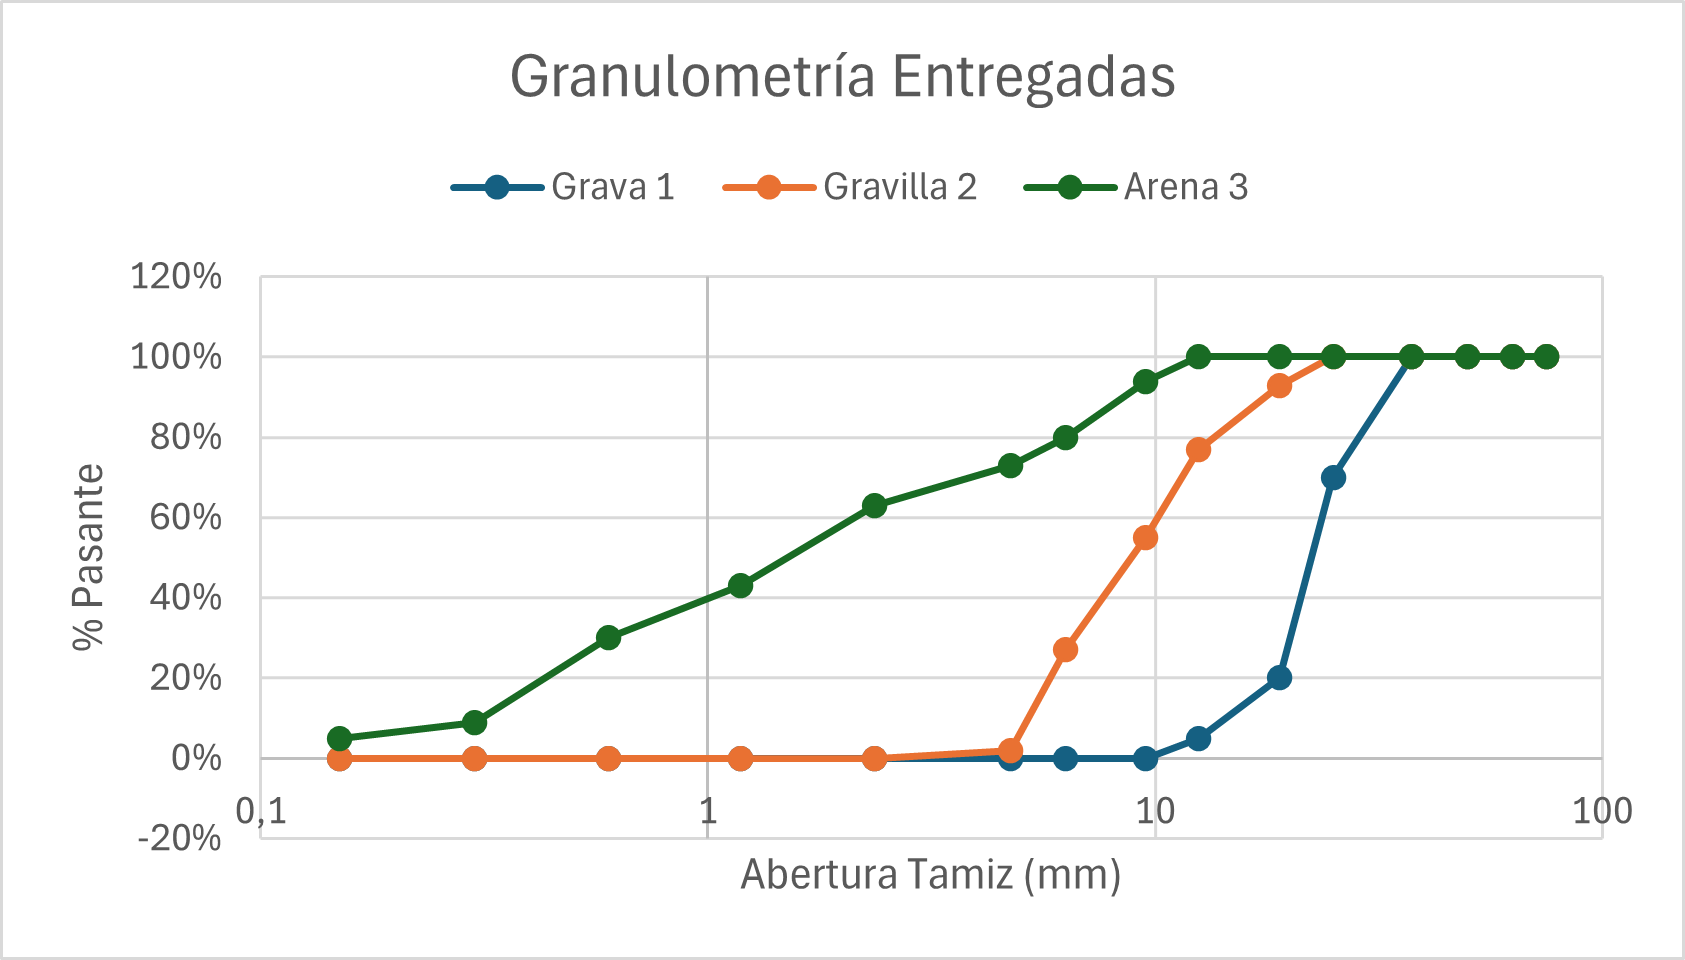
\includegraphics[width=0.8\textwidth]{GRAFICOS/granu_inicial.png}
    \caption{Curvas granulométricas iniciales de los áridos.}
\end{figure}

Posteriormente, en base a la norma, se graficaron las curvas asociadas al Dm 10mm, ya que por condición inicial el TMA es 9,5mm y se obtuvo la curva de granulometría sugerida, la cual es el promedio entre las curvas A, B, C y D. La figura se muestra a continuación.

\begin{figure}[H]
    \centering
    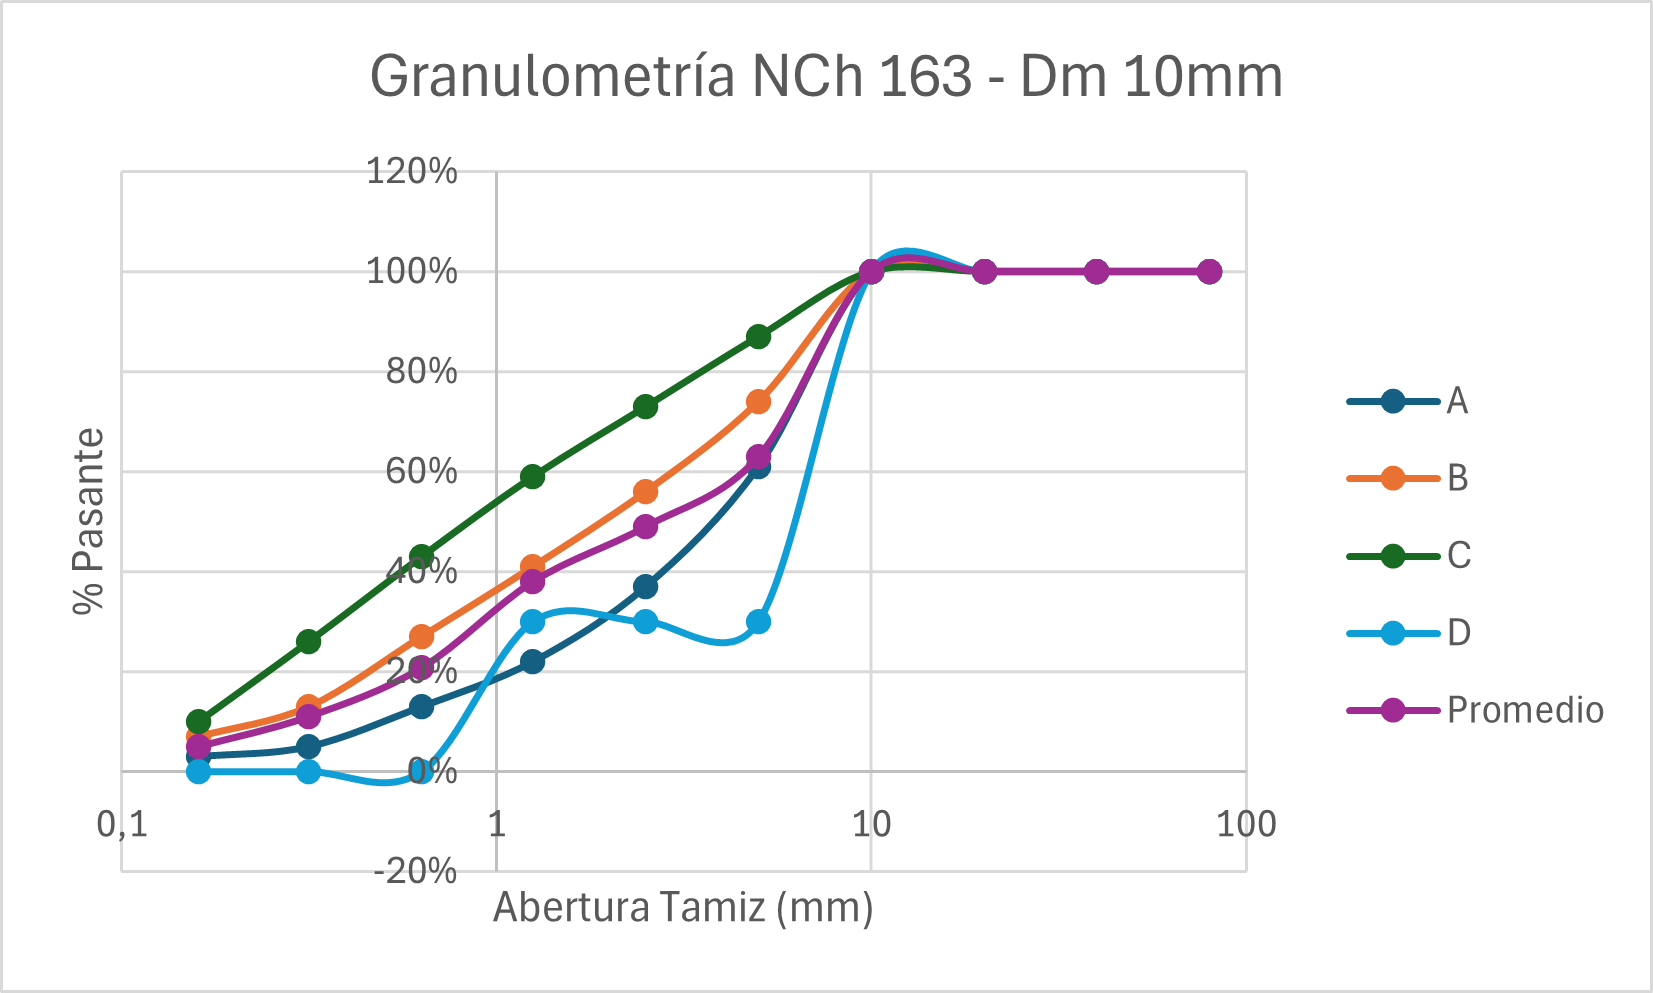
\includegraphics[width=0.8\textwidth]{GRAFICOS/NCh163.png}
    \caption{Curva de granulometría sugerida para Dm 10mm.}
\end{figure}

Una vez obtenida la curva sugerida, se procede a la optimización granulométrica en base a la norma. Este proceso consistió en interpolar los \% pasantes combinados de nuestra mezcla a los tamices indicados en la norma para poder compararlos. Finalmente, se realizó una iteración con la función objetivo de Excel para poder llevar la curva combinada a la sugerida, la cual varía los \% de cada árido hasta que la diferencia entre ambas curvas sea igual a 0, manteniendo las condiciones y requerimientos iniciales, dando como resultado la curva optimizada.
\\\\
Además, dadas las condiciones iniciales, las condiciones de ejecución en obra, el elemento a hormigonar, el tipo de hormigón y la clase de exposición en obra, se procedió a obtener el contenido de agua y cemento necesario para poder calcular el factor K, el cual corresponde a la masa total de áridos en estado SSS. Con estos datos, se pudo reemplazar en la ecuación de balance de volumen y obtener las proporciones finales de cada árido a utilizar en la mezcla optimizada.

\begin{table}[H]
\centering
\caption{Factor K y masas de agregados - TMA}
\label{tab:factor_k_tma}
\begin{tabular}{|l|r|c|}
\hline
\textbf{Volumen} & \textbf{1} & \textbf{m$^{3}$} \\ \hline
w          & 177,98     & kg/m$^{3}$ \\ \hline
c          & 286,14  & kg/m$^{3}$ \\ \hline
K          & 1942,28  & kg/m$^{3}$ \\ \hline
Grava 1    & 504,38  & kg/m$^{3}$ \\ \hline
Gravilla 2 & 481,04  & kg/m$^{3}$ \\ \hline
Arena 3    & 956,85  & kg/m$^{3}$ \\ \hline
\end{tabular}
\end{table}

La siguiente tabla muestra los \% finales obtenidos para la ponderación de cada árido y la figura muestra la curva optmizada comparada con la curva sugerida. Se puede notar que la diferencia entre ambas esta minimizada.

\begin{table}[H]
\centering
\caption{Ponderaciones finales de los áridos utilizando método de Banda.}
\begin{tabular}{|l|c|}
\hline
\textbf{Material} & \textbf{Ponderación Final (\%)} \\ \hline
Grava 1     & 25,97 \\ \hline
Gravilla 2  & 24,77 \\ \hline
Arena 3     & 49,26 \\ \hline
\end{tabular}
\end{table}

\begin{figure}[H]
    \centering
    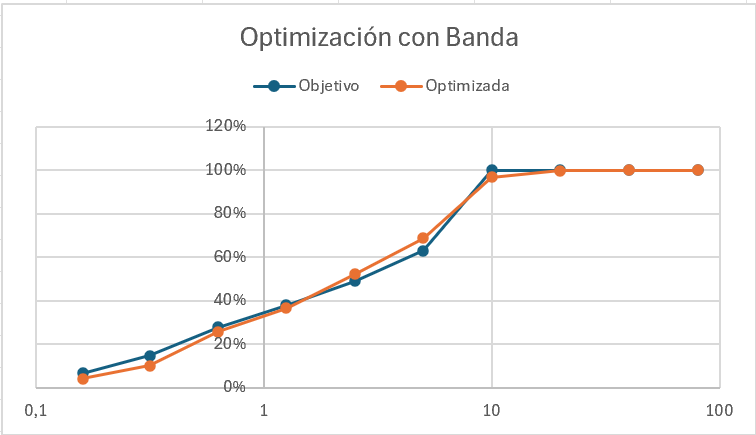
\includegraphics[width=0.8\textwidth]{GRAFICOS/opti_banda.png}
    \caption{Curva granulométrica optimizada comparada con la curva sugerida TMA.}
\end{figure}

Finalmente, obtenidas las proporciones finales de cada árido y la granulometría optimizada, se corrigió cada cantidad por humedad y rendimiento, obtuviendo los siguientes resultados.
\begin{table}[H]
\centering
\captionsetup{justification=centering}
\caption{Corrección por humedad (TMA = 9{,}5 mm).}
\label{tab:correccion-humedad}
\setlength{\tabcolsep}{6pt}
\renewcommand{\arraystretch}{1.15}
\small
\makebox[\textwidth][c]{%
\begin{tabular}{@{} c c c c c c @{}} % columnas centradas y sin padding lateral
\toprule
\textbf{Material} &
\textbf{SSS (kg/m$^{3}$)} &
\textbf{Agua absorción (kg/m$^{3}$)} &
\textbf{Peso seco (kg/m$^{3}$)} &
\textbf{Agua total (kg/m$^{3}$)} &
\textbf{Áridos húmedos (kg/m$^{3}$)} \\
\midrule
Cemento                 & 286,14 & --    & --     & --    & 286,14 \\
Agua de amasado         & 177,98 & --    & --     & --    & 86,83  \\
Agua de abs.\ de áridos & --     & 23,52 & --     & -23,52& --     \\
\midrule
Grava 1                 & 504,38 & -6,47 & 497,91 & 19,92 & 517,82 \\
Gravilla 2              & 481,04 & -5,70 & 475,34 & 38,03 & 513,36 \\
Arena 3                 & 956,86 & -11,35& 945,51 & 56,73 & 1002,24\\
\midrule
\textbf{Peso hormigón (kg)} & \textbf{2406,41} &  &  &  & \textbf{2406,41} \\
\bottomrule
\end{tabular}%
}
\end{table}


\begin{table}[H]
\centering
\caption{Rendimiento de mezcla y factor de densidad}
\label{tab:rend-y-factor}
\small
\setlength{\tabcolsep}{6pt}
\renewcommand{\arraystretch}{1.15}

\begin{subtable}[t]{0.38\textwidth}
\centering
\caption{Densidades}
\label{tab:factor-rendimiento}
\begin{tabular}{lr}
\toprule
\textbf{Concepto} & \textbf{Valor} \\
\midrule
Densidad teórica & 2406,41 \\
Densidad real    & 2350 \\
Factor de densidad          & 0,97656 \\
\bottomrule
\end{tabular}
\end{subtable}
\begin{subtable}[t]{0.58\textwidth}
\centering
\caption{Corrección por Rendimiento}
\label{tab:rendimiento}
\begin{tabular}{lrrr}
\toprule
 & \textbf{Teórico} & \textbf{Real} & \textbf{Corregida} \\
\midrule
Cemento   & 286,14 & 279,44 & 286,14 \\
Agua      & 86,83 & 84,80 & 86,83 \\
Agregados & 2033,43 & 1985,76 & 1977,02 \\
Densidad  & 2406,41 & 2350 & 2350 \\
\bottomrule
\end{tabular}
\end{subtable}

\end{table}


\subsection{Fuller - Thompson}

En esta sección se realizó una nueva optimización granulométrica utilizando el método de Fuller-Thomposon. Esta curva sigue una distribución de potencia, como se expresa a continuación:

\begin{equation}
    P(D) = 100 \times (\frac{D}{D_{max}})^n
\end{equation}

Donde $P(D)$ es el \% que pasa por el tamiz de diámetro $D$, $D_{max}$ es el tamaño máximo del árido (TMA) y $n$ es el exponente que define la forma de la curva, el cual, según Fuller, tiene un valor de 0,5 para hormigones.

El objetivo es lograr que la curva de los áridos combinados con los \% optimizados sea lo más parecida a la curva sugerida por el método Fuller - Thompson, minimizando su diferencia. La curva sugerida se obtiene reemplazando la dosificación sugerida por la NCH 163 en la fórmula anterior.  

A continuación se muestran los resultados obtenidos.

\begin{table}[H]
\centering
\caption{Ponderaciones finales de los áridos utilizando Fuller-Thompson.}
\begin{tabular}{|l|c|}
\hline
\textbf{Material} & \textbf{Ponderación Final (\%)} \\ \hline
Grava 1     & 28,52 \\ \hline
Gravilla 2  & 23,07 \\ \hline
Arena 3     & 48,42 \\ \hline
\end{tabular}
\end{table}

\begin{figure}[H]
    \centering
    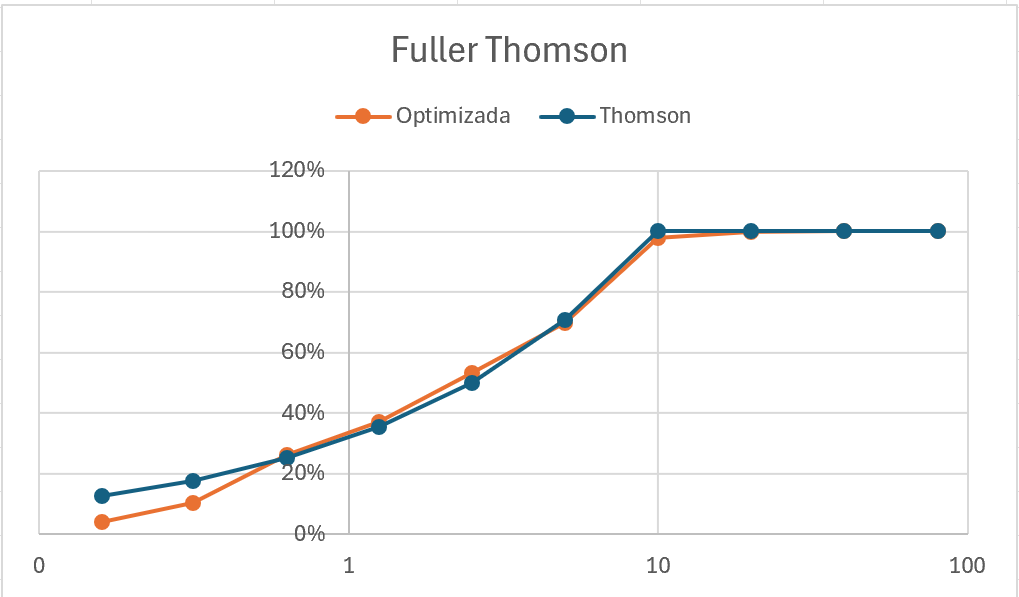
\includegraphics[width=0.8\textwidth]{GRAFICOS/fuller_thompson.png}
    \caption{Curva granulométrica optimizada comparada con la curva Fuller-Thompson.}
\end{figure}

Se puede analizar que los resultados son similares a los obtenidos por el método de Banda, donde hay una cantidad similar de grava y gravilla con una dosis considerable de arena. Además, se puede observar que la diferencia de cada punto de la curva optimizada con la sugerida también es mínima. Las diferencias notorias se pueden ver más adelante, en el análisis de la curva Tarántula. 

Posteriormente, se obtuvieron las masas requeridas de agua, cemento y agregados corregidas, utilizando las condiciones y requerimientos iniciales.

\begin{table}[H]
\centering
\captionsetup{justification=centering}
\caption{Corrección por humedad — Fuller - Thompson.}
\label{tab:correccion-humedad-thomson}
\setlength{\tabcolsep}{6pt}
\renewcommand{\arraystretch}{1.15}
\small
\makebox[\textwidth][c]{%
\begin{tabular}{@{} l r r r r r @{}} % l + 5 numéricas
\toprule
\textbf{Material} & \textbf{SSS (kg/m$^{3}$)} & \textbf{Agua absorción (kg/m$^{3}$)} &
\textbf{Peso seco (kg/m$^{3}$)} & \textbf{Agua total (kg/m$^{3}$)} &
\textbf{Áridos húmedos (kg/m$^{3}$)} \\
\midrule
Cemento                 & 286,14 & --            & --       & --        & 286,14 \\
Agua de amasado         & 177,98    & --            & --       & -23,53& 88,65 \\
Agua de abs.\ de áridos & --          & 23,53     & --       & -112,86 & -- \\
\midrule
Grava 1                 & 552,97 & -7,10  & 545,87 & 21,83   & 567,71 \\
Gravilla 2              & 447,36 & -5,30  & 442,05 & 35,36   & 477,42 \\
Arena 3                 & 938,88 & -11,13 & 927,75 & 55,67   & 983,41 \\
\midrule
\textbf{Peso hormigón (kg)} & \textbf{2403,34} &  &  &  & \textbf{2403,34} \\
\bottomrule
\end{tabular}%
}
\end{table}

\begin{table}[H]
\centering
\caption{Rendimiento (Thomson) y factor de densidad}
\label{tab:rendimiento-factor-thomson}
\small
\setlength{\tabcolsep}{6pt}
\renewcommand{\arraystretch}{1.15}

\begin{subtable}[t]{0.58\textwidth}
\centering
\caption{Rendimiento (Thomson)}
\begin{tabular}{lrrr}
\toprule
 & \textbf{Teórico} & \textbf{Real} & \textbf{Corregida} \\
\midrule
Cemento   & 286,14 & 279,79 & 286,14 \\
Agua      & 88,65 & 86,69 & 88,65 \\
Agregados & 2028,54 & 1983,52 & 1975,20 \\
Densidad  & 2403,34 & 2350 & 2350 \\
\bottomrule
\end{tabular}
\end{subtable}
\hfill
\begin{subtable}[t]{0.38\textwidth}
\centering
\caption{Densidades y factor}
\begin{tabular}{lr}
\toprule
\textbf{Concepto} & \textbf{Valor} \\
\midrule
Densidad teórica & 2403,33 \\
Densidad real    & 2350 \\
Factor           & 0,9778 \\
\bottomrule
\end{tabular}
\end{subtable}

\end{table}

\begin{table}[H]
\centering
\caption{Factor K - Fuller - Thompson}
\label{tab:factor-k-thomson}
\setlength{\tabcolsep}{6pt}
\renewcommand{\arraystretch}{1.15}
\small
\begin{tabular}{|l|r|c|}
\hline
\textbf{Volumen} & \textbf{1} & \textbf{m$^{3}$} \\ \hline
w          & 177,98     & kg/m$^{3}$ \\ \hline
c          & 286,15  & kg/m$^{3}$ \\ \hline
K          & 1939,21  & kg/m$^{3}$ \\ \hline
Grava 1    & 552,97  & kg/m$^{3}$ \\ \hline
Gravilla 2 & 447,36  & kg/m$^{3}$ \\ \hline
Arena 3    & 938,88  & kg/m$^{3}$ \\ \hline
\end{tabular}
\end{table}

\subsection{Curva Tarántula}

En esta sección se analizarán los resultados obtenidos utilizando el método de la curva Tarántula para evaluar su trabajabilidad. Es importante mencionar que las porporciones finales de cada árido en cada método de optimización fueron ajustadas para que cumplan las condiciones de la curva Tarántula.

\begin{figure}[H]
    \centering
    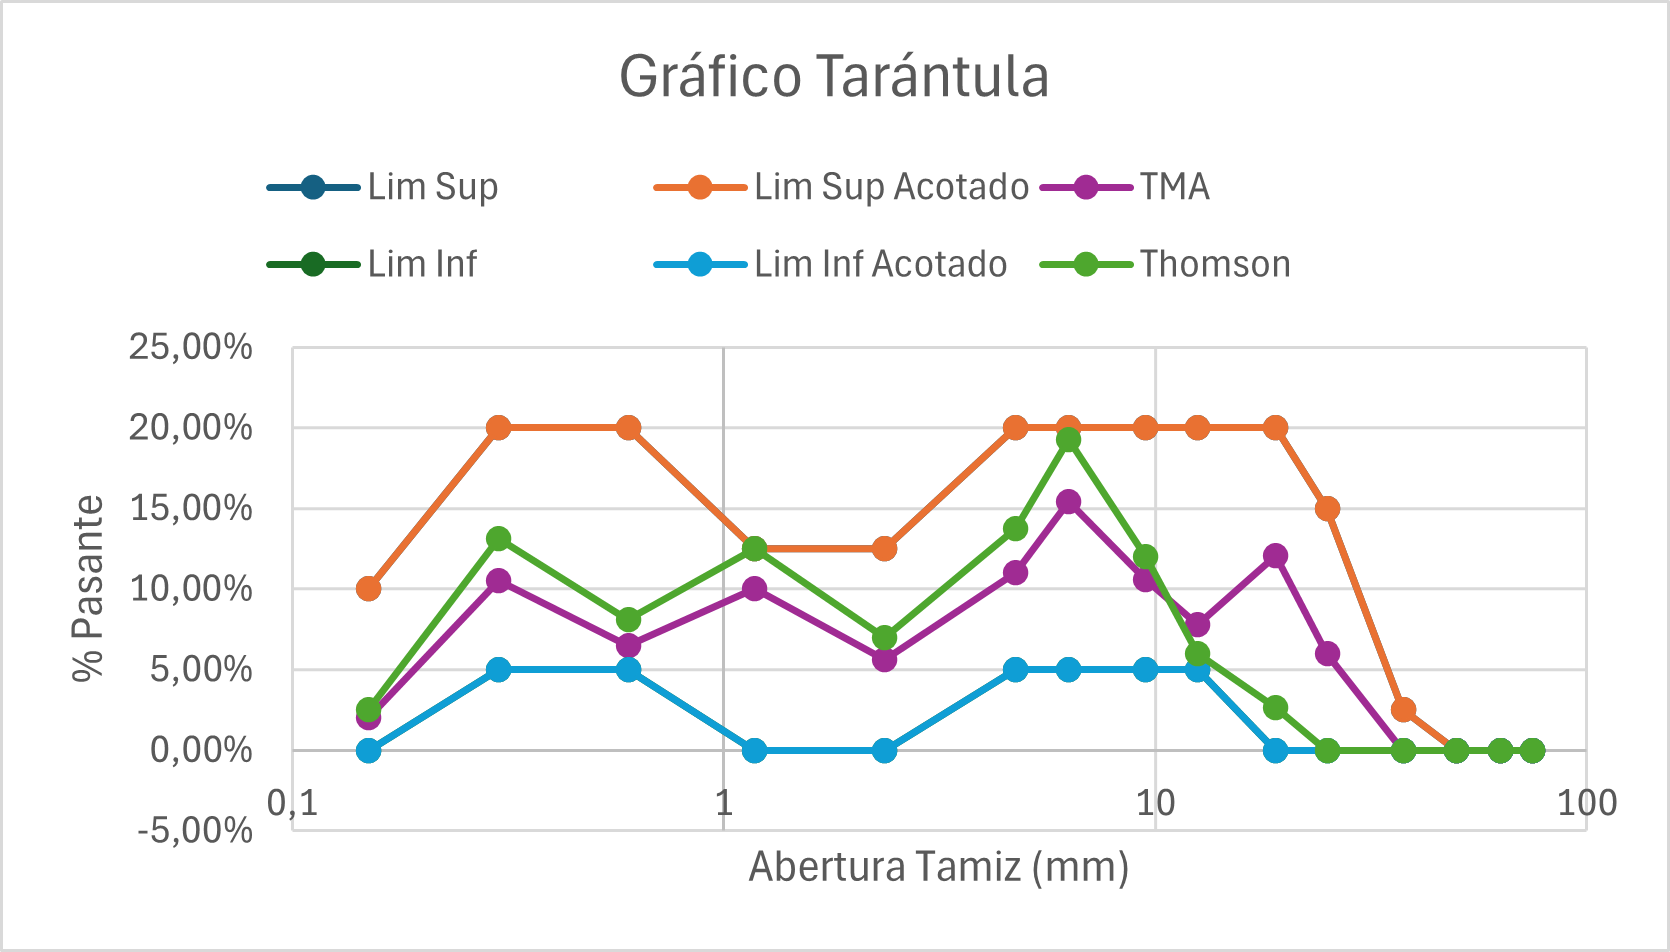
\includegraphics[width=0.8\textwidth]{GRAFICOS/tarantula.png}
    \caption{Curva Tarántula optimizada.}
\end{figure}


El gráfico compara los límites de la Curva Tarántula (superior e inferior) con las curvas combinadas de los diseños TMA y Thompson para TMA = \(9{,}5\) mm. En conjunto, ambas mezclas se mantienen dentro del sobre acotado en todo el rango de tamices, lo que es indicio de buena trabajabilidad, estabilidad y óptimo para la construcción.

En la fracción de finos \((<0{,}3~\mathrm{mm})\), las curvas se sitúan por encima del límite inferior y abajo del límite superior. Esto evita el déficit de finos, que se manifiesta como textura áspera, falta de cohesión y sangrado, y, a la vez, reduce el riesgo de pegajosidad y exudación asociado a un exceso de partículas muy finas. La distribución observada en esta zona favorece una pasta trabajable.

En el rango de arena gruesa \((0{,}6\text{–}2{,}36~\mathrm{mm})\) se aprecia un máximo controlado alrededor de \(1\text{–}2~\mathrm{mm}\), siempre por debajo del límite superior. Esta proporción es deseable porque promueve el deslizamiento entre partículas, estabiliza el asentamiento y contribuye a una respuesta reológica predecible en estado fresco.

Los áridos gruesos \((2{,}36\text{–}4{,}75~\mathrm{mm})\) mantienen una continuidad granulométrica dentro de la Tarántula. La cercanía de las curvas a dicho centro sugiere una buena distribución granular, con baja probabilidad de vacíos intermedios.

La fracción gruesa \((\ge 9{,}5~\mathrm{mm})\) se mantiene baja, coherente con el TMA de \(3/8''\) y con una dosificación dominada por arena y gravilla fina. Esto explica la compatibilidad general con la Curva Tarántula. Al limitar el tamaño máximo, se reduce la exigencia de pasta para envolver partículas grandes y se mejora la movilidad del hormigón.

Al comparar los diseños, la curva Thomson resulta levemente más fina por debajo de \(1\text{–}1{,}18~\mathrm{mm}\) y muy similar a TMA entre \(2{,}36\) y \(4{,}75~\mathrm{mm}\). La diferencia en la zona de finos es consistente con un empaque algo más suave y con los ajustes por humedad y rendimiento aplicados durante la dosificación. Por su parte, la curva TMA se mantiene próxima a Thomson dentro del sobre acotado; por ello, ambas alternativas son técnicamente válidas y la selección final puede fundarse en la disponibilidad de áridos, la respuesta observada en mezcla de prueba y los requisitos de puesta en obra.

Desde el punto de vista reológico, el cumplimiento sistemático del sobre acotado sugiere mezclas cohesivas, estables y bombeables. El pico controlado en \(0{,}6\text{–}2{,}36~\mathrm{mm}\) favorece la retención del asentamiento y el empleo eficiente de aditivo reductor de agua, sin necesidad de incrementar la fracción de finos más allá de lo recomendable.

En caso de ser necesario un ajuste fino en obra, se propone actuar de manera dirigida sobre los intervalos granulométricos críticos. Si la mezcla se percibe pegajosa, conviene trasladar entre 1 y 2 puntos porcentuales desde \(<0{,}3~\mathrm{mm}\) hacia \(0{,}6\text{–}1{,}18~\mathrm{mm}\) o \(1{,}18\text{–}2{,}36~\mathrm{mm}\). Por el contrario, si se detecta pérdida de cohesión o sangrado, es preferible añadir aproximadamente 1 punto porcentual a \(<0{,}3~\mathrm{mm}\) retirándolo de \(2{,}36\text{–}4{,}75~\mathrm{mm}\). Tras cada intervención, debe verificarse nuevamente el cumplimiento del sobre acotado de la Curva Tarántula para asegurar que la mezcla permanezca dentro de los márgenes establecidos.

En síntesis, las curvas combinadas TMA y Thomson cumplen la Curva Tarántula en todo el espectro de tamices, con desempeño especialmente favorable en \(0{,}6\text{–}2{,}36~\mathrm{mm}\). Estos resultados respaldan la viabilidad reológica y la aptitud de bombeo del diseño con TMA \(3/8''\), a la vez que reducen el riesgo de segregación y exudación en las condiciones de ejecución previstas.


REVISAR




\section{Anexos}

\subsection{Tamizado de Agregados iniciales}

%---------------------- TABLA: GRAVA 1 ----------------------
\begin{table}[H]
\centering
\caption{Análisis granulométrico – Grava 1}
\label{tab:grava1}
\small
\begin{tabular}{|c|c|c|c|c|}
\hline
\textbf{Apertura (mm)} & \textbf{ASTM} & \textbf{Retenido [g]} & \textbf{Retenido [\%]} & \textbf{Pasa [\%]} \\ \hline
75   & 3"      & 0   & 0\%  & 100\% \\ \hline
63   & 2 1/2"  & 0   & 0\%  & 100\% \\ \hline
50   & 2"      & 0   & 0\%  & 100\% \\ \hline
37,5 & 1 1/2"  & 60  & 6\%  & 94\%  \\ \hline
25   & 1"      & 320 & 32\% & 62\%  \\ \hline
19   & 3/4"    & 480 & 48\% & 14\%  \\ \hline
12,5 & 1/2"    & 60  & 6\%  & 8\%   \\ \hline
9,5  & 3/8"    & 80  & 8\%  & 0\%   \\ \hline
6,3  & 1/4"    & 0   & 0\%  & 0\%   \\ \hline
4,75 & N°4     & 0   & 0\%  & 0\%   \\ \hline
2,36 & N°8     & 0   & 0\%  & 0\%   \\ \hline
1,18 & N°16    & 0   & 0\%  & 0\%   \\ \hline
0,6  & N°30    & 0   & 0\%  & 0\%   \\ \hline
0,3  & N°50    & 0   & 0\%  & 0\%   \\ \hline
0,15 & N°100   & 0   & 0\%  & 0\%   \\ \hline
\textbf{Residuo} &     & 0   & -    & -     \\ \hline
\textbf{TOTAL}  &     & 1000& 100\%& -     \\ \hline
\end{tabular}
\end{table}

%---------------------- TABLA: GRAVILLA 2 ----------------------
\begin{table}[H]
\centering
\caption{Análisis granulométrico – Gravilla 2}
\label{tab:gravilla2}
\small
\begin{tabular}{|c|c|c|c|c|}
\hline
\textbf{Apertura (mm)} & \textbf{ASTM} & \textbf{Retenido [g]} & \textbf{Retenido [\%]} & \textbf{Pasa [\%]} \\ \hline
75   & 3"      & 0   & 0\%  & 100\% \\ \hline
63   & 2 1/2"  & 0   & 0\%  & 100\% \\ \hline
50   & 2"      & 0   & 0\%  & 100\% \\ \hline
37,5 & 1 1/2"  & 0   & 0\%  & 100\% \\ \hline
25   & 1"      & 0   & 0\%  & 100\% \\ \hline
19   & 3/4"    & 50  & 5\%  & 95\%  \\ \hline
12,5 & 1/2"    & 350 & 35\% & 60\%  \\ \hline
9,5  & 3/8"    & 120 & 12\% & 48\%  \\ \hline
6,3  & 1/4"    & 280 & 28\% & 20\%  \\ \hline
4,75 & N°4     & 80  & 8\%  & 12\%  \\ \hline
2,36 & N°8     & 120 & 12\% & 0\%   \\ \hline
1,18 & N°16    & 0   & 0\%  & 0\%   \\ \hline
0,6  & N°30    & 0   & 0\%  & 0\%   \\ \hline
0,3  & N°50    & 0   & 0\%  & 0\%   \\ \hline
0,15 & N°100   & 0   & 0\%  & 0\%   \\ \hline
\textbf{Residuo} &     & 0   & -    & -     \\ \hline
\textbf{TOTAL}  &     & 1000& 100\%& -     \\ \hline
\end{tabular}
\end{table}

%---------------------- TABLA: ARENA 3 ----------------------
\begin{table}[H]
\centering
\caption{Análisis granulométrico – Arena 3}
\label{tab:arena3}
\small
\begin{tabular}{|c|c|c|c|c|}
\hline
\textbf{Apertura (mm)} & \textbf{ASTM} & \textbf{Retenido [g]} & \textbf{Retenido [\%]} & \textbf{Pasa [\%]} \\ \hline
75   & 3"      & 0   & 0\%  & 100\% \\ \hline
63   & 2 1/2"  & 0   & 0\%  & 100\% \\ \hline
50   & 2"      & 0   & 0\%  & 100\% \\ \hline
37,5 & 1 1/2"  & 0   & 0\%  & 100\% \\ \hline
25   & 1"      & 0   & 0\%  & 100\% \\ \hline
19   & 3/4"    & 0   & 0\%  & 100\% \\ \hline
12,5 & 1/2"    & 0   & 0\%  & 100\% \\ \hline
9,5  & 3/8"    & 0   & 0\%  & 100\% \\ \hline
6,3  & 1/4"    & 40  & 4\%  & 96\%  \\ \hline
4,75 & N°4     & 280 & 28\% & 68\%  \\ \hline
2,36 & N°8     & 130 & 13\% & 55\%  \\ \hline
1,18 & N°16    & 170 & 17\% & 38\%  \\ \hline
0,6  & N°30    & 110 & 11\% & 27\%  \\ \hline
0,3  & N°50    & 170 & 17\% & 10\%  \\ \hline
0,15 & N°100   & 60  & 6\%  & 4\%   \\ \hline
\textbf{Residuo} &     & 40  & -    & -     \\ \hline
\textbf{TOTAL}  &     & 1000& 100\%& -     \\ \hline
\end{tabular}
\end{table}


\bibliographystyle{plainnat}  % Estilo de la bibliografía (puedes cambiarlo a otro si prefieres)
\bibliography{ref.bib}  % Nombre del archivo .bib

\end{document}